% 中文内部稿。正式投稿前需翻译为英文，并补全作者、单位和基金信息。
\documentclass{article}
\usepackage{spconf,amsmath,amssymb,graphicx}
\usepackage{booktabs}
\usepackage[UTF8,fontset=fandol]{ctex}
\usepackage[hidelinks]{hyperref}
\usepackage{url}

\makeatletter
\def\abstract{\begin{center}{\bf 摘要\vspace{-.5em}\vspace{0pt}}\end{center}}
\def\endabstract{\par}
\def\keywords{\vspace{.5em}{\bfseries 关键词}---\,\relax}
\def\endkeywords{\par}
\makeatother

\title{面向双耳360$^\circ$ DOA分类的结构化线索分解与紧凑融合}
\name{作者姓名（待补充）}
\address{作者单位与联系邮箱（待补充）}

\begin{document}
\ninept
\maketitle

\begin{abstract}
双耳360$^\circ$定位需要同时利用耳间差异与方向相关频谱结构，但这些信息具有不同的物理含义和统计形式：ILD/IPD直接描述左右耳差异，局部耳间相干性描述两耳观测的一致程度，而双耳幅度谱还保留源频谱与HRTF频谱着色。紧凑模型若在高维输入端统一处理这些异质信息，有限容量将同时承担差异提取、上下文建模和线索整合。本文据此提出一种“先保持结构、后低维融合”的72类静态DOA网络。共享编码器提取两耳幅度谱表示，并以均值、带符号差值和绝对差值显式组织双耳关系；两个低维分支分别编码ILD/IPD方向线索值与局部相干性，随后由单层BiGRU和注意力池化聚合。在当前7,776样本的KEMAR测试协议上，模型以$0.153\,\mathrm{M}$参数和$0.391\,\mathrm{GFLOPs}$获得96.51\%准确率与2.46$^\circ$环形MAE。消融结果表明，幅度谱上下文在显式线索之外仍提供互补信息，独立相干性编码与分离式线索编码也优于对应的移除或合并变体。结果支持按线索结构分配有限建模能力可形成有竞争力的性能--效率权衡。
\end{abstract}

\begin{keywords}
双耳声源定位，到达方向估计，双耳空间线索，耳间相干性，轻量神经网络
\end{keywords}

\section{引言}
\label{sec:intro}

双耳声源定位根据左右耳信号估计声源方向，是空间音频、听觉辅助与机器人听觉的重要基础。本文聚焦静态单说话人的完整水平面定位：输入为2秒双通道语音，输出为覆盖$[-180^\circ,180^\circ)$的72类片段级方位预测。该任务并非普通的72类识别，因为类别首尾在几何上相邻，且两耳观测同时受到头部遮挡、耳廓滤波、反射声与背景噪声影响；模型既要命中离散方向，也要控制圆周上的大角度错误与计算成本。

双耳线索在退化条件下并不同步失效。ILD和IPD分别刻画两耳幅度比与相位关系，但反射声会将直达声与延迟副本叠加，加性噪声也会以不同强度污染各时频区域\cite{blauert1997,may2011}。若只观察耳间差异，前后方向还可能产生相近观测，即经典的锥形混淆；区分它们需要结合耳廓与头部引入的方向相关频谱着色\cite{blauert1997}。因此，显式耳间差异、局部两耳一致性和幅度谱上下文承担相关但不同的角色。

现有方法可直接从波形或完整时频表示学习空间映射\cite{vecchiotti2019}，也可先构造GCC-PHAT、ILD/IPD或相对传递函数等物理线索\cite{knapp1976,tokala2025}。高容量时频网络减少手工假设，但计算随频率分辨率、序列长度和隐藏维度增长；把全部特征沿通道维直接拼接，则要求同一编码器同时处理频谱结构、方向差异和相干性。这里不能未经对照断言统一编码必然失败，真正可检验的问题是：在紧凑预算下，是否应先用与线索结构匹配的低成本路径编码，再进行融合？

本文将有限容量分配给三种结构。两耳幅度谱先由共享编码器映射到可比较空间，再构造交换不变的均值和绝对差值，以及交换变号的带符号差值。方向线索分支编码$\mathrm{ILD}$、$\sin(\mathrm{IPD})$与$\cos(\mathrm{IPD})$，避免直接相位在$-\pi$与$\pi$处的数值跳变；相干性分支则保留归一化互谱中不同于线索取值的信息。三路表示不执行显式门控或置信度校准，而是在112维特征层融合后由单层BiGRU聚合。

现有证据支持三点贡献：（1）给出一种$0.153\,\mathrm{M}$参数、$0.391\,\mathrm{GFLOPs}$的结构化紧凑网络，在当前静态KEMAR协议上获得96.51\%准确率和2.46$^\circ$环形MAE；（2）仅保留显式线索的变体仍达到95.95\%准确率，而完整模型将MAE由2.94$^\circ$降至2.46$^\circ$，支持幅度谱上下文提供互补证据；（3）移除相干性或合并线索编码均增加MAE，支持先保持线索结构、再融合的设计判断。本文不声称绝对精度最优，也不将结论外推到未见HRTF、真实录音或移动声源。

\section{相关工作}
\label{sec:related}

传统双耳定位主要利用差异线索与频谱线索。双耳时间差、IPD和ILD描述声波到达两耳的时间、相位和能量差异\cite{blauert1997}，GCC-PHAT则通过跨通道相关峰估计传播时延\cite{knapp1976}。这些线索具有物理解释，但单凭耳间差异并不总能消除前后混淆；混响和扩散噪声还会使观测偏离直达声条件。耳间相干性是归一化互谱幅度的一类统计量，可描述局部两耳关系的一致程度，但其数值不天然等于校准的可靠概率\cite{may2011}。

数据驱动方法使用卷积、循环或端到端结构学习双耳信号到方向的映射。Vecchiotti等直接从原始波形学习双耳定位\cite{vecchiotti2019}，Tokala等以GCC-PHAT和卷积循环网络处理噪声语音定位\cite{tokala2025}。本文实现SDEL-style、FN-SSL-style、DP-RTF-style和BiL-style四类项目内适配模型；这些名称不代表原论文官方结果。与统一高维建模或只使用显式线索不同，本文保留可解释的ILD/IPD，同时用共享幅度谱编码补充上下文，并把统一时序建模推迟到低维融合之后。研究目标是验证这种容量分配的性能--效率权衡，而非宣称绝对精度超过全部基线。

\section{所提方法}
\label{sec:method}

\begin{figure*}[t]
    \centering
    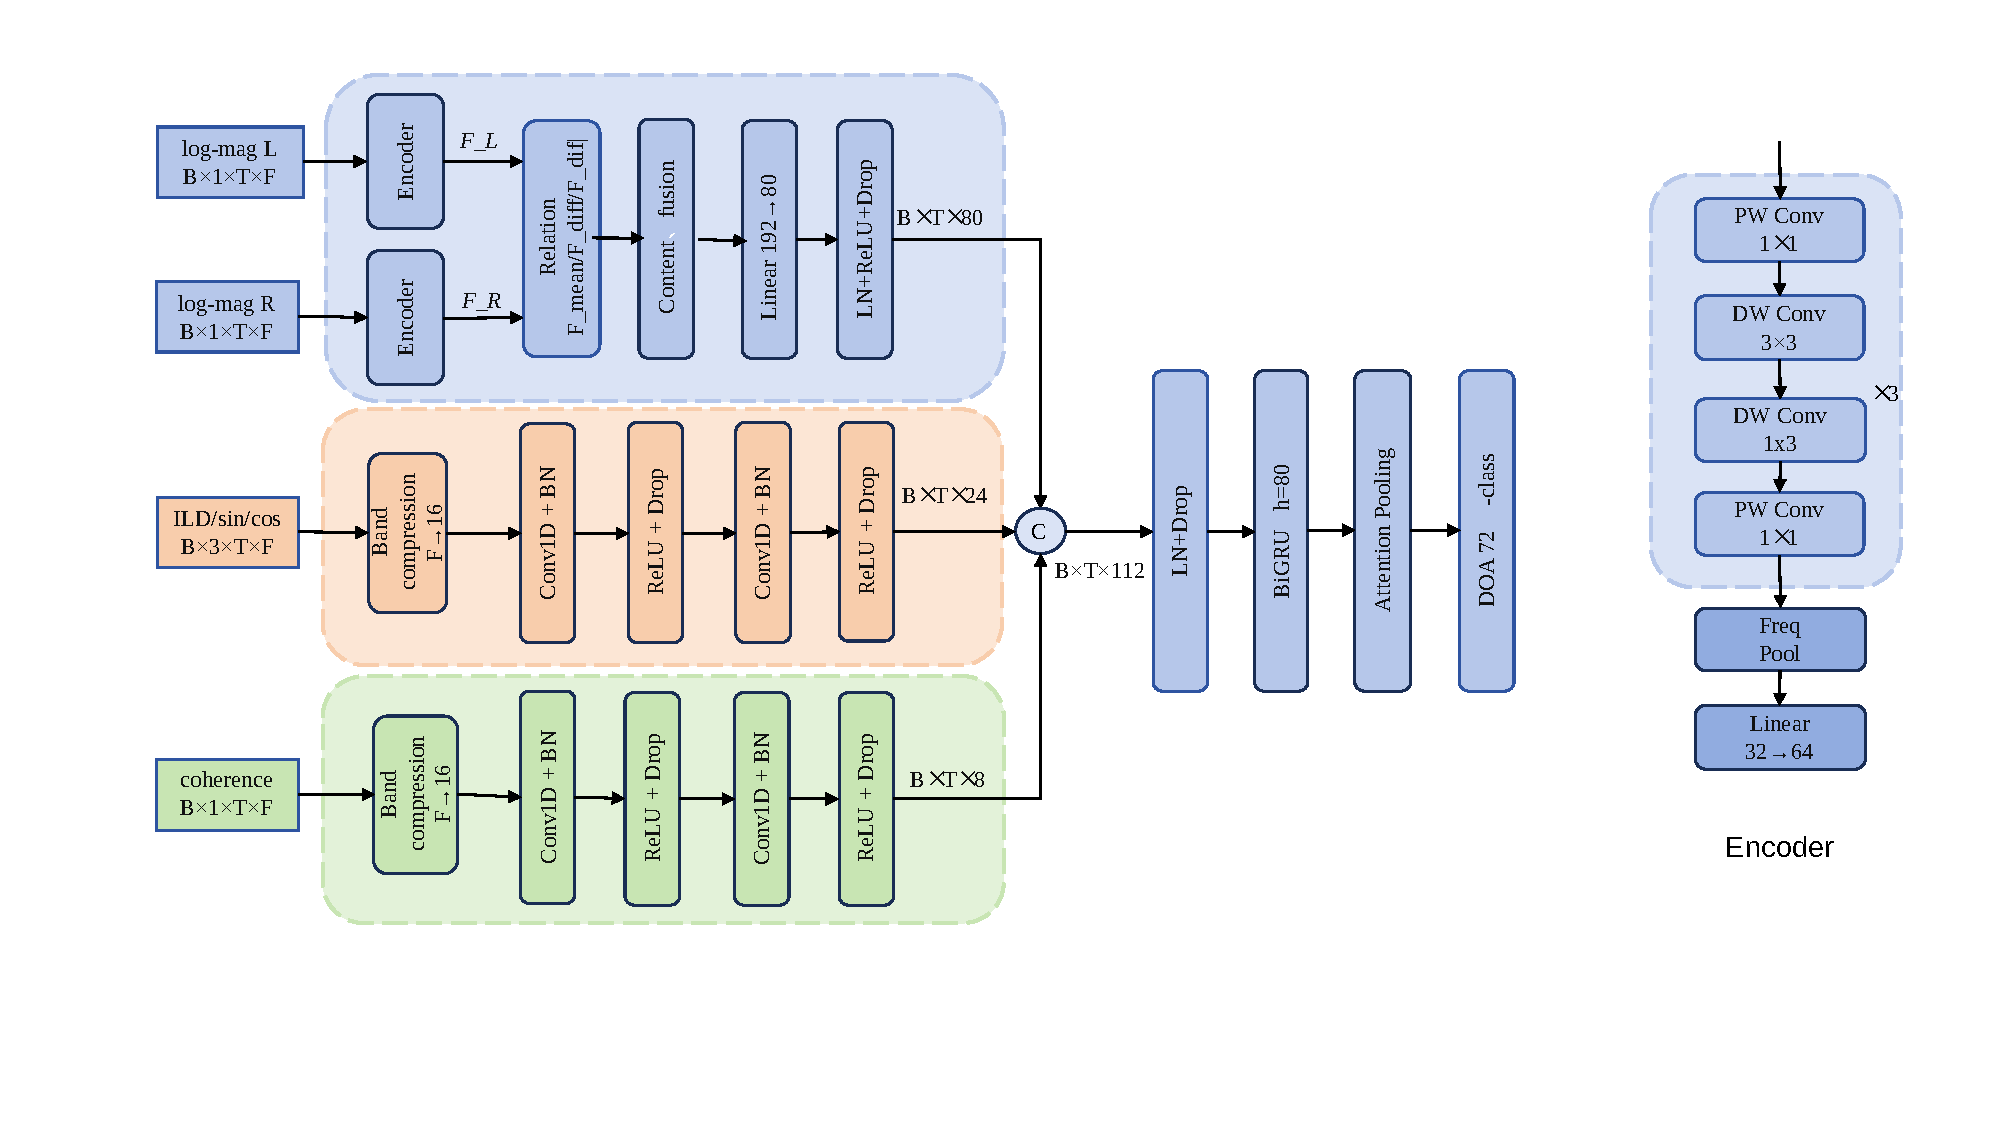
\includegraphics[width=0.98\textwidth,trim=74 98 48 35,clip]{figures/model_architecture.pdf}
    \caption{所提结构化线索分解网络。幅度谱上下文、方向线索值与相干性分别编码，在112维特征层拼接后进行时序聚合。右侧给出共享轻量幅度谱编码器的单个阶段。}
    \label{fig:model}
\end{figure*}

图\ref{fig:model}给出整体结构。方法遵循三项原则：对同类型的左右耳幅度谱共享编码；对已显式计算的方向线索先压缩频带、再低成本建模；对取值空间不同的ILD/IPD与相干性分别编码，最后统一聚合。该结构先验是否有效由移除与合并消融检验，而不由模块命名预设。

\subsection{任务定义与双耳特征}

设左右耳波形为$x_L,x_R\in\mathbb{R}^{N}$，其复数短时傅里叶变换为$X_L(t,f)$和$X_R(t,f)$。标签$y\in\{0,\ldots,71\}$对应固定方位
\begin{equation}
    \theta_y=-180^\circ+5^\circ y .
\end{equation}
模型输出72维logits，不执行连续角度回归。两耳幅度谱上下文输入为$M_e=\log(|X_e|+\epsilon)$，$e\in\{L,R\}$。显式方向线索定义为
\begin{align}
 D &=20\log_{10}\frac{|X_L|+\epsilon}{|X_R|+\epsilon}, \\
 \Phi &=\angle(X_LX_R^*),\qquad
 \mathbf{Q}_v=[D,\sin\Phi,\cos\Phi].
\end{align}
用$\sin\Phi$和$\cos\Phi$表示IPD，可避免物理相邻的$-\pi$与$\pi$在标量轴上发生跳变。局部耳间相干性为
\begin{equation}
 C=\frac{|\mathcal{S}\{X_LX_R^*\}|}
 {\sqrt{\mathcal{S}\{|X_L|^2\}\mathcal{S}\{|X_R|^2\}}+\epsilon},
\end{equation}
其中$\mathcal{S}$为采用反射填充的$5\times3$频率--时间局部平均，$C$最终截断至$[0,1]$。该归一化互谱统计不同于相位取值或幅度比；本文将这种差异作为独立编码的动机，而不把$C$解释为校准概率。

\subsection{幅度谱上下文流}

幅度谱上下文流保留显式ILD/IPD没有完整表达的信息。单耳对数幅度谱既包含源谱包络，也包含HRTF、房间和噪声造成的频谱着色，因而不是“纯内容特征”。如图\ref{fig:model}所示，同一轻量编码器$E_c$处理左右耳对数幅度谱：
\begin{equation}
 \mathbf{F}_L=E_c(M_L),\quad \mathbf{F}_R=E_c(M_R),\quad
 \mathbf{F}_e\in\mathbb{R}^{T\times64}.
\end{equation}
$E_c$包含通道数为16、24和32的三个阶段；每阶段由$1\times1$逐点卷积、$3\times3$深度卷积、步长$(1,2)$的$1\times3$深度卷积及$1\times1$逐点卷积组成，仅沿频率轴降采样。自适应频率平均池化与线性投影产生64维逐帧表示。共享权重不仅减少参数，也把$\mathbf{F}_L$和$\mathbf{F}_R$置于同一特征坐标系，使逐维关系具有可比基础；由于没有非共享编码器对照，本文不声称共享本身必然提高精度。

两耳表示通过确定性关系组合：
\begin{equation}
 \mathbf{R}_c=\left[\frac{\mathbf{F}_L+\mathbf{F}_R}{2},\,
 \mathbf{F}_L-\mathbf{F}_R,\,|\mathbf{F}_L-\mathbf{F}_R|\right].
\end{equation}
这些关系具有明确的耳交换行为：均值和绝对差值保持不变，带符号差值改变符号。因此，表示同时暴露共同成分、差异强度与左右方向性，而无需后续网络先从任意拼接中重新构造这些基础关系。拼接结果经线性层、层归一化、ReLU和dropout投影为$\mathbf{H}_c\in\mathbb{R}^{T\times80}$。本文只验证整个上下文流的作用，尚未证明三个关系项分别不可替代或模型具备严格耳交换等变性。

\subsection{线索分支、时序融合与目标函数}

ILD/IPD已由左右耳复谱直接计算，线索分支无需重新发现两耳差异，而只需整合其频率与时间分布。方向线索值和相干性先分别将257个频点平均池化为16个频带，再经过两层核大小为3的一维时间卷积，输出$\mathbf{H}_v\in\mathbb{R}^{T\times24}$和$\mathbf{H}_r\in\mathbb{R}^{T\times8}$。这种先压缩频率、后执行时序卷积的顺序限制了计算开销；但当前没有频带数对照，不能声称16带划分本身提高抗噪性。相干性单独编码是因为归一化互谱幅度与ILD/IPD的取值空间不同，而不是预先把它定义为“可信/不可信”标签。实现仅拼接$\mathbf{H}_v$与$\mathbf{H}_r$，不利用相干性生成门控或显式重标定方向线索。

三路表示经层归一化与dropout得到
\begin{equation}
 \mathbf{Z}=\mathrm{Drop}\!\left(\mathrm{LN}([\mathbf{H}_c,\mathbf{H}_v,\mathbf{H}_r])\right)
 \in\mathbb{R}^{T\times112}.
\end{equation}
融合被推迟到各分支压缩为帧级表示之后，因此时序头处理112维输入而非完整多通道时频平面。单层BiGRU在每个方向使用80个隐藏单元；双向建模适用于当前整段可见的离线分类，但不满足因果实时约束。两层打分网络$g(\cdot)$计算注意力权重$a_t=\exp(g(\mathbf{u}_t))/\sum_j\exp(g(\mathbf{u}_j))$，并以$\bar{\mathbf{u}}=\sum_ta_t\mathbf{u}_t$完成片段级聚合。训练损失为
\begin{equation}
 \mathcal{L}=\mathrm{CE}_{\mathrm{LS}}(\mathbf{o},y)
 +0.3\,\mathrm{CE}(\mathbf{o}_{\mathrm{fb}},y_{\mathrm{fb}}),
\end{equation}
其中主任务标签平滑系数为0.1，前后辅助头仅用于训练；本文没有辅助头开关消融，故不将其列为独立贡献。

\begin{table*}[!t]
\centering
\caption{不同SNR下的静态定位结果。每项为三次运行平均Accuracy（\%）/环形MAE（$^\circ$）；不包含clean条件。}
\label{tab:bysnr}
\small
\begin{tabular}{lccccc}
\toprule
方法 & 10 dB & 5 dB & 0 dB & $-5$ dB & $-10$ dB \\
\midrule
所提模型 & 98.89 / 0.87 & 98.56 / 1.37 & 97.33 / 2.12 & 94.42 / 3.63 & 90.15 / 6.30 \\
SDEL-style & \textbf{99.07} / 1.20 & \textbf{99.05} / \textbf{0.92} & \textbf{97.99} / \textbf{1.74} & \textbf{95.47} / 3.44 & \textbf{91.77} / \textbf{5.35} \\
FN-SSL-style & 98.71 / 1.22 & 98.61 / 1.29 & 97.38 / 2.11 & 95.45 / \textbf{2.88} & 91.20 / 6.04 \\
DP-RTF-style & 98.05 / 2.59 & 97.25 / 3.07 & 95.99 / 4.33 & 94.39 / 5.21 & 89.09 / 7.51 \\
BiL-style & 97.81 / 2.33 & 96.63 / 3.59 & 94.80 / 4.66 & 91.05 / 7.51 & 84.67 / 12.74 \\
\bottomrule
\end{tabular}
\end{table*}

\begin{table}[!t]
\centering
\caption{复杂度与完整测试集结果。定位指标为三次运行均值。}
\label{tab:complexity}
\resizebox{\columnwidth}{!}{%
\begin{tabular}{lccccc}
\toprule
方法 & 参数/M & MACs/G & FLOPs/G & Acc./\% & MAE/$^\circ$ \\
\midrule
所提模型 & \textbf{0.153} & \textbf{0.195} & \textbf{0.391} & 96.51 & 2.46 \\
SDEL-style & 0.926 & 0.701 & 1.402 & \textbf{97.18} & \textbf{2.18} \\
FN-SSL-style & 0.659 & 32.843 & 65.687 & 96.75 & 2.33 \\
DP-RTF-style & 0.877 & 4.107 & 8.215 & 95.49 & 4.22 \\
BiL-style & 0.865 & 1.559 & 3.117 & 93.97 & 5.41 \\
\bottomrule
\end{tabular}}
\end{table}

\begin{table}[!t]
\centering
\caption{完整测试集上的消融结果（均值$\pm$总体标准差）。}
\label{tab:ablation}
\begin{tabular}{lcc}
\toprule
变体 & Accuracy/\% $\uparrow$ & MAE/$^\circ$ $\downarrow$ \\
\midrule
完整模型 & \textbf{96.51$\pm$0.10} & \textbf{2.46$\pm$0.06} \\
移除幅度谱上下文流 & 95.95$\pm$0.24 & 2.94$\pm$0.16 \\
移除相干性分支 & 95.96$\pm$0.14 & 2.95$\pm$0.03 \\
合并线索编码器 & 96.16$\pm$0.18 & 3.05$\pm$0.19 \\
\bottomrule
\end{tabular}
\end{table}

\section{实验}
\label{sec:experiments}

\subsection{数据、设置与指标}

静态双耳数据由LibriSpeech语音\cite{panayotov2015}、MIT KEMAR HRTF\cite{gardner1995}和SofaMyRoom房间模拟器\cite{barumerli2021}生成，并叠加DEMAND场景噪声\cite{thiemann2013}。训练、验证和测试集分别包含36,000、7,200和7,776条2秒样本。训练与验证噪声为TMETRO、PCAFETER和OOFFICE，SNR从$[-10,10]\,\mathrm{dB}$均匀采样；测试使用未见的TBUS、NPARK和SPSQUARE，并包含clean、10、5、0、$-5$和$-10\,\mathrm{dB}$。测试覆盖六个固定房间，目标RT60为0.30--0.80秒，声源距离约1--2米。所有集合均使用同一KEMAR，因此不评估跨HRTF泛化。

输入采样率为$16\,\mathrm{kHz}$，STFT使用512点DFT、400点Hann窗和160点帧移。模型使用AdamW，初始学习率$5\times10^{-4}$、权重衰减$10^{-4}$、batch size 64、dropout 0.2，余弦调度最低学习率$10^{-5}$，最多100个epoch，早停耐心值15。主结果和消融报告随机种子42、43和44的均值；FN-SSL-style三次运行的辅助头设置不完全一致，因此只将其作为当前适配实现的参考。

Accuracy为72类完全命中率。预测类别$\hat y$先映射为$\hat\theta=-180^\circ+5^\circ\hat y$，再计算环形角距离
\begin{equation}
 d_{\mathrm{circ}}=\left|((\hat\theta-\theta+180^\circ)\bmod360^\circ)-180^\circ\right|.
\end{equation}
MAE为$d_{\mathrm{circ}}$的样本均值，衡量离散类别预测的圆周角误差，不代表连续回归精度。复杂度以参数量、MACs和FLOPs报告。

\subsection{不同SNR下的定位性能}

表\ref{tab:bysnr}比较五个含噪条件，以观察噪声增强时的退化趋势。所提模型的准确率从$10\,\mathrm{dB}$下的98.89\%降至$-10\,\mathrm{dB}$下的90.15\%，MAE由0.87$^\circ$增至6.30$^\circ$。SDEL-style在多数条件下具有更强的绝对性能；所提模型则在全部SNR上均优于当前DP-RTF-style与BiL-style的准确率和MAE。相对FN-SSL-style不存在覆盖所有条件的一致优势，因此证据支持的是渐进退化和性能--效率权衡，而非定位精度最优。

\subsection{性能--复杂度权衡}

表\ref{tab:complexity}比较完整测试集结果与复杂度。所提模型是当前比较中参数量、MACs和FLOPs最低的模型。相较SDEL-style，其参数量和FLOPs分别减少83.5\%和72.1\%，代价是准确率低0.67个百分点、MAE高0.28$^\circ$；相较FN-SSL-style，其FLOPs约为$1/168$，准确率低0.24个百分点、MAE高0.13$^\circ$。这些结果支持紧凑性，但低FLOPs不能替代尚未测量的目标硬件延迟、内存和能耗。

\subsection{消融实验}

表\ref{tab:ablation}检验三类结构分解。移除幅度谱上下文流后，准确率下降0.56个百分点且MAE增加0.48$^\circ$，说明显式ILD/IPD之外仍存在互补的幅度谱上下文。移除相干性分支后，两项变化分别为$-0.55$个百分点和$+0.49^\circ$，支持独立相干性编码在当前组合中有益。将方向线索与相干性送入同一个合并编码器后，MAE增加0.59$^\circ$，表明分离编码优于所测试的合并实现。由于尚无配对显著性检验，本文不将这些差异描述为统计显著。

三项消融形成一条相互约束的证据链。无幅度谱上下文的线索模型仍达到95.95\%准确率，说明显式ILD/IPD已承担大部分方向判别；加入幅度谱上下文与相干性后，完整模型进一步降低圆周角误差，表明三类输入并非完全冗余；合并线索编码未带来更低误差，则支持在当前预算与对照范围内先保持线索结构、再低维融合。该解释描述观察到的模型行为，不等同于证明每个分支内部恢复了预设声学变量。

当前测试协议存在语音划分限制：6,784个唯一测试语音路径中有4,868个也出现在训练集。方位标签由独立声学渲染产生，因而该现象不等同于已证实的标签泄漏；但它阻止本文声称说话人或语句无关泛化。完整的speech-disjoint基线与消融重训仍在进行，本文不混用尚未闭环的新协议结果。

\section{结论}

本文面向双耳360$^\circ$水平DOA分类，研究如何按照线索结构分配有限表示容量。方法以共享编码器组织两耳幅度谱关系，以低维分支分别处理ILD/IPD方向线索与耳间相干性，再以112维表示和单层BiGRU完成片段级融合。在当前模拟KEMAR静态协议上，模型以$0.153\,\mathrm{M}$参数和$0.391\,\mathrm{GFLOPs}$取得96.51\%准确率与2.46$^\circ$环形MAE。复杂度对比支持其性能--效率工作点，消融则显示显式线索承担主要方向判别，幅度谱上下文与相干性提供互补信息，分离编码优于所测合并实现。当前结论受固定KEMAR、模拟环境和语音路径重叠限制，不能外推到未见HRTF、真实录音、移动声源或实时部署。后续首先完成speech-disjoint全套评测，再引入实测BRIR与目标设备延迟验证。

\bibliographystyle{IEEEbib}
\bibliography{refs_zh}

\end{document}
